%% LyX 2.0.0 created this file.  For more info, see http://www.lyx.org/.
%% Do not edit unless you really know what you are doing.
\documentclass[a4paper,british]{article}
\usepackage{mathptmx}
\usepackage[T1]{fontenc}
\usepackage[latin9]{inputenc}
\usepackage{babel}
\usepackage{covington}
\usepackage{amsmath}
\usepackage{graphicx}
\usepackage[unicode=true,
 bookmarks=true,bookmarksnumbered=false,bookmarksopen=false,
 breaklinks=true,pdfborder={0 0 0},backref=false,colorlinks=false]
 {hyperref}

\makeatletter

%%%%%%%%%%%%%%%%%%%%%%%%%%%%%% LyX specific LaTeX commands.
\pdfpageheight\paperheight
\pdfpagewidth\paperwidth

%% Because html converters don't know tabularnewline
\providecommand{\tabularnewline}{\\}
%% A simple dot to overcome graphicx limitations
\newcommand{\lyxdot}{.}


%%%%%%%%%%%%%%%%%%%%%%%%%%%%%% Textclass specific LaTeX commands.
\newenvironment{lyxlist}[1]
{\begin{list}{}
{\settowidth{\labelwidth}{#1}
 \setlength{\leftmargin}{\labelwidth}
 \addtolength{\leftmargin}{\labelsep}
 \renewcommand{\makelabel}[1]{##1\hfil}}}
{\end{list}}

%%%%%%%%%%%%%%%%%%%%%%%%%%%%%% User specified LaTeX commands.
\usepackage{acl-hlt2011}

\newcommand{\BM}[1]{\textbf{BM: #1}}
\newcommand{\MB}[1]{\textbf{MB: #1}}
\newcommand{\MP}[1]{\textbf{MP: #1}}
\newcommand{\ES}[1]{\textbf{ES: #1}}

\makeatother

\begin{document}

\title{Evaluating a Minimally-Supervised Web-Corpus of Hiberno-English}


\author{Brian Murphy\\
 Centre for Mind/Brain Sciences, \\
University of Trento\\
38068 Rovereto (TN), Italy \\
\texttt{brian.murphy@unitn.it} \And Egon Stemle\\
 Centre for Mind/Brain Sciences, \\
University of Trento\\
38068 Rovereto (TN), Italy \\
\texttt{egon.stemle@unitn.it}}
\maketitle
\begin{abstract}
Small, manually assembled corpora may be available for less dominant
languages and dialects, but producing web-scale resources remains
challenging. Even when considerable quantities of text are present
on the web, finding this text, and distinguishing it from related
languages in the same region can be challenging. For example less
dominant variants of English (e.g. New Zealander, Singaporean, Canadian,
Irish, South African) may be found under their respective national
domains, but will be partially mixed with Englishes of the British
and US varieties, perhaps through syndication of journalism, or the
local reuse of text by multinational companies. Less formal dialectal
usage may be scattered more widely over the internet through mechanisms
such as wiki or blog authoring. Here we automatically construct a
corpus of Hiberno-English (English as spoken in Ireland) using a variety
of methods: filtering by national domain, filtering by orthographic
conventions, and bootstrapping from a set of Ireland-specific terms
(slang, place names, organisations). We evaluate the national specificity
of the resulting corpora by measuring the incidence of topical terms,
and several grammatical constructions that are particular to Hiberno-English.
The results show that domain filtering is very effective for isolating
text that is topic-specific, and orthographic classification can exclude
some non-Irish texts, but that selected seeds are necessary to extract
considerable quantities of more informal, dialectal text.


\end{abstract}

\section*{Introduction}

For less dominant language variants, corpora are usually painstakingly
constructed by hand. This results in high quality collections of text,
classified and balanced by genre, register and modality. But the process
is time-consuming and expensive, and results in relatively small resources.
For example the International Corpus of English (ICE) project has
already resulted in the publication of corpora covering ten dialects
of English, following a common schema, but the individual corpora
are limited to approximately one million words.

An alternative is to use automatic methods to harvest corpora from
the Web. Identification of major languages is a robust technology,
and where the regional boundaries of a language or dialect correspond
closely to a national top-level internet domain, very large collections
(of several billion words) can now can be produced easily, with close
to no manual intervention \cite{wackycorpora2009}. The methods can
also deal with some issues of text quality found on the web, successfully
extracting coherent pieces of running text from web pages (i.e. discarding
menu text, generic headings, copyright and other legal notices), reducing
textual duplication, and identifying spam, portal pages and other
files that do not contain linguistically interesting text. 

However for language variants that do not have their own domain (e.g.
Scots, Bavarian), it is less clear that such web corpora can be automatically
constructed. Smaller or politically less dominant countries that do
have their own domain (e.g. Belgium, New Zealand), may also find the
language of their {}``national'' web strongly influenced by other
language varieties, for example through syndication of journalistic
articles, or materials published by foreign companies.

In this paper we use a minimally supervised method \cite{BaroniSilvia2004,wackycorpora2009}
to quickly and cheaply build corpora of Hiberno-English (English as
spoken in Ireland), which are many times larger than the biggest publicly
collection currently available (ICE-Ireland, \cite{kallenKirk2007iceIreland}).
We investigate several combinations of strategies (based on domain
names, and on regional variations in vocabulary and orthography) to
distinguish text written in this minor language variant from related
dominant variants (US and UK English). We validate the specificity
of the resulting corpora by measuring the incidence of Ireland-specific
language, both topically (the frequency with which Irish regions and
organisations are mentioned), and structurally, by the presence of
grammatical constructions that are particular to Hiberno-English.

The results show that filtering by national domain is very effective
in identifying text that deals with Irish topics, but that the grammar
of the resulting text is largely standard, apparently indistinguishable
from UK and US English. In contrast, using a set of seed terms tailored
to the language variant (Irish slang, names of Ireland-based organisations,
loanwords from Irish Gaelic), yields text which is much more characteristic
of Hiberno-English usage. The application of a British/American spelling
filter can further boost the incidence of both topical and structural
features of the language variant.

The paper proceeds as follows: in the next section we introduce Hiberno-English,
situating it relative to other variants of English, and concentrating
on the characteristic features that will be used as metrics of {}``Irishness''
of text retrieved from the Web. Next we describe the process by which
several candidate corpora of Hiberno-English were constructed (section
\ref{sec:Constructing-a-Web-Corpus}), and the methods we used to
quantify incidence of distinctive usage (section \eqref{sec:Evaluating-Variety-Specificity}).
In the final two sections we compare the incidence of these markers
with those found in corpora of other variants of English (UK, US),
and a hand-crafted corpus of Hiberno-English (ICE-Ireland), and reflect
on the wider applicability of these methods to variants of other languages
and orthographies.


\section{Structures and Lexicon of Hiberno-English\label{sec:Structures-and-Lexicon}}

Hiberno-English differs in a range of ways from other varieties of
English. In broad terms it can be grouped with British English, in
that the its lexicon, grammar and orthographic conventions are more
similar to that of Great Britain, than to that of North America. For
example with lexical variants such as \emph{bumper/fender, rubbish
bin/trash can, lift/elevator }and \emph{zed/zee} it shares the former
British usage rather than the later American usage, though there are
exceptions (in Irish usage the North Americans term \emph{truck }is
replacing the British \emph{lorry}). Similarly in syntax it tends
to follow British conventions, for instance \emph{He's familiar with
X }rather than \emph{X is familiar to him}, \emph{write to me} rather
than \emph{write me }and the acceptability of singular verbal marking
with group subjects, as in \emph{the team are pleased}  -- though
there are counterexamples again, in that Irish English tends to follow
American dialects in dispensing with the \emph{shall/will }distinction.
Most obviously, Irish writing uses British spellings rather than American
spellings.

However, there are still dialectal differences between Irish and British
English. Beyond the usual regional differences that one might find
between the words used in different parts of England, the English
spoken in Ireland is particularly influenced by the Irish language
(Gaelic, \emph{Gaeilge}) \cite{kirkKallen2007celtICEIreland}. While
English is the first language of the overwhelming majority of residents
of Ireland (estimates of Irishmother-tongue speakers are of the order
of 50,000, or about 1\% of the population), Irish retains status as
the first official language of the Republic of Ireland, maintained
as a core subject at all levels of school education, and through state-maintained
radio and television channels. As recently as the early 19th century,
Irish was the majority language, and so many traces of it remain in
modern Hiberno-English, in the form of Irish loan-words (e.g. \emph{sl�n}
`goodbye', \emph{gaelscoil} `Irish (speaking) school'), Anglicizations
(e.g. `gansey', jumper, from Irish \emph{geansa�}), and composites
(e.g. `jackeen', a pejorative term for Dubliners, combining the Irish
diminutive \emph{-�n} with the English `Jack'). 

In this paper we take a series of characteristic terms and structures
from Hiberno-English, mostly inspired by \cite{kirkKallen2007celtICEIreland},
and use them as markers of the Irishness of the text we assemble from
the web. While there are many more interesting grammatical differences
between Hiberno-English and other variants (e.g. perfective use of
the simple present: \emph{I know that family for years}), we restrict
ourselves to those that can be easily isolated in a corpus through
searching of plain text, or of shallow structural patterns (part of
speech). 

The first marker we use is to measure the incidence of a set of terms
that are topically related to Ireland: proper names of Ireland-based
organisations, and geographical terms, and the method for assembling
this list is described in section \ref{sec:Evaluating-Variety-Specificity}.

The most simple structure that we use as a marker of Hiberno-English
is the contraction \emph{I amn't }(\emph{I'm not} or \emph{I ain't}
in other varieties). The next is the {}``after'' perfective, which
often expresses immediacy, and a negative outcome \eqref{afterConstruction}.
\begin{examples}
\item \label{afterConstruction}I'm after losing my wallet\\
`I just lost my wallet'
\end{examples}
A further structure that is novel from the point of view of other
variants of English is a particular use of verbs that take a complement
that expresses a question (most commonly \emph{ask, wonder, see} and
\emph{know}), without the use of a complementizer such as \emph{if
}or \emph{whether} and with an inversion of subject-verb order (typical
of interrogatives) \eqref{embeddedInversion}. 
\begin{examples}
\item \label{embeddedInversion}I wonder is he coming''\\
`I wonder if/whether he is coming'
\end{examples}
Finally we consider the expanded usage of reflexive pronouns in Hiberno-English,
where they may be used for emphasis, in any argument position, and
without being anaphorically bound, as is usually required. Here we
limit ourselves to subject position reflexives, which can be identified
from word order patterns, without any deeper semantic analysis \eqref{subjectReflexive}. 
\begin{examples}
\item \label{subjectReflexive}himself is in big trouble\\
`he is in big trouble'
\end{examples}
With the exception of the \emph{amn't }contraction, all of these phenomena
are demonstrated by \cite{kirkKallen2007celtICEIreland} to be common
in the ICE-Ireland corpus, though somewhat less common in Northern
Irish portion of that collection, and to be very rare or completely
absent in the ICE-GB corpus of the English of Britain. Significantly,
these constructions are found predominantly in the spoken language
portion of the ICE-Ireland corpus, suggesting that speakers are perhaps
aware that they are not {}``standard'' English, and so not considered
appropriate in the written register.


\section{Constructing a Web-Corpus of Hiberno-English\label{sec:Constructing-a-Web-Corpus}}

Within the WaCky initiative (Web-as-Corpus kool ynitiative) \cite{Wacky2006}
a community of linguists and information technology specialists developed
a set of tools to selectively crawl sections of the Web, and then
process, index and search the resulting data. Contributions like BootCaT
\cite{BaroniSilvia2004}, an iterative procedure to bootstrap specialised
corpora and terms from the Web, have been successfully used in a range
of projects: first in the construction of the \emph{WaCky corpora},
a collection of very large (>1 billion words) corpora of English (ukWaC),
German (deWaC) and Italian (itWaC); and subsequently by other groups,
e.g. noWaC and jpWaC \cite{wackycorpora2009,NoWaC2010,JpWaC2009}. 

Here we use BootCaT to build five prototype corpora of Hiberno-English,
and evaluate the dialect-specificity of these corpora by measuring
the incidence of proper terms and constructions that are associated
with this language variant. Additionally, we use ukWaC as the de-facto
standard British English Web corpus, and construct a medium size web-corpus
of the US domain to represent American usage. Each corpus is preprocessed
and formatted for the IMS Open Corpus Workbench (CWB, \cite{Christ1994,cwb}),
a generic query engine for large text corpora that was developed for
applications in computational lexicography. 

BootCaT first takes a set of manually assembled seed terms, these
(possibly multi-word) terms are randomly combined and, then, used
as search queries against a Web search engine; the HTML documents
of the top results are downloaded and cleaned to extract running text
and discard all web-markup. Preprocessing and formatting for the CWB
consists of tokenising, lemmatising, and part-of-speech tagging the
corpus, and, then, converting the result into CWB's internal format;
we replicated the processing stages employed for ukWaC (see REF, for
more details). 

The construction of the six corpora differs in three dimensions: 
\begin{description}
\item [{Seeds:}] two seed sets were used namely, an Hiberno-English one,
and the original ukWaC list (mid-frequency terms from the British
National Corpus; \cite{Burn95bnc}).
\item [{TLDs:}] two types of top-level internet domain (TLD) restrictions
were imposed during (or after) the construction of the corpora; either
no restriction was imposed, or a corpus was filtered by a specific
national TLD.
\item [{Spelling:}] two types of spelling filter were imposed; either none,
or an `orthographic convention factor' (OCF) was calculated, and a
corpus was filtered accordingly.
\end{description}
The IE seeds contained 81 seed terms, gathered using one author's
native intuition, and words indicated as being specific to Irish English
by the Oxford English Dictionary, and from various Web pages about
Hiberno-English. 76 single-word and 5 two-word terms were used falling
into three main categories: Irish place names, regional variant terms
(mostly slang), and load words from Irish Gaelic (many being state
institutions). The full listing of terms is given here: 
\begin{description}
\item [{Place~names:}] Dublin, Galway, Waterford, Drogheda, Antrim, Derry,
Kildare, Meath, Donegal, Armagh, Wexford, Wicklow, Louth, Kilkenny,
Westmeath, Offaly, Laois, Belfast, Cavan, Sligo, Roscommon, Monaghan,
Fermanagh, Carlow, Longford, Leitrim, Navan, Ennis, Tralee, Leinster,
Connaught, Munster, Ulster
\item [{Regional~variants:}] banjaxed (wrecked), craic (fun), fecking
(variant of fucking), yoke (thing), yer man/one/wan (that man/woman),
culchie (country dweller), da (father), footpath (pavement), gaff
(home), gobshite (curse), gurrier (young child), jackeen (Dubliner),
jacks (toilet), janey mac (exclamation), jaysus (variant of exclamation
{}``jesus''), kip (sleep; hovel), knacker (Traveller, gypsy), knackered
(wrecked), langer (penis; idiot), langers/langered (drunk), scallion
(spring onion), skanger (disgusting person), strand (beach, seaside),
scuttered (drunk), boreen (small road), gob (mouth; spit), eejit (variant
of idiot), lough (lake), fooster (dawdle), barmbrack (traditional
Hallow'een cake), shebeen (unlicensed bar), bogman (contry dweller),
old one (old lady), quare (variant queer), gansey (pullover)
\item [{Loan~words:}] garda, garda� (police), taoiseach (prime minister),
d�il (parliament), Sl�inte ({}``cheers''), Gaeltacht (Irish speaking
areas), Seanad (senate), T�naiste (deputy prime minister), ceol ((traditional
Irish) music), sl�n ({}``goodbye''), gr� (affection, love for),
gaelscoil (Irish speaking school)
\end{description}
These seed terms were combined into a set of 3000 3-tuple search queries,
i.e. two-word terms were enclosed in inverted commas to form one single
term for the search engine; 2440 3-tuples with only single-word terms,
534 with only 2 single-word terms, 25 with only 1 single-word term,
and 1 with 3 two-word terms were used. The UK seeds were the ones
used during the construction of the ukWaC corpus and they were randomly
combined into 3000 3-tuple search queries.

No TLD restriction means that the search engine was not instructed
to return search results within a specific domain, and hence, documents
originate from .com, .ie, .uk, etc. but also from .de and potentially
any other. A restriction implies that the documents can only originate
from - in our case - one TLD.

No spelling filter means that nothing was done. The OCF indicates
the degree to which terms within a document are predominantly spelt
according to one predefined word list than to another. It is calculated
as the proportion of the difference between the overlaps to the sum
of the overlaps. To simplify matters, we utilised a spell-checker
to return the list of known words from a document, this corresponds
to checking a document for spelling errors and only keeping the non-erroneous
words. In our case we used an en\_GB dictionary, an en\_US one, and
the two together. The three lists yield the needed numbers of words
only known by one of the two dictionaries, and, hence unknown by the
other dictionary, and the ratio in the range of $[-1,+1]$ can be
calculated.

The search engine we used for all queries was Yahoo \cite{yahoo};
for all search queries English results were requested, that is we
relied on the search engine's built-in language identification algorithm%
\footnote{This restriction is very effective at distinguishing non-English from
English content, but returns content from all English variants.%
}, and from all search queries the top 10 results were used. Cleaning
of the Web pages (termed \emph{boilerplate removal}) was accomplished
by BootCaT's implementation of the \cite{FinnKushmerickSmyth2001}
BTE method; it strives to extract the main body of a Web page, i.e.
the largest contiguous text area with the least amount of intervening
non-text elements (HTML tags), and discards the rest.

Three corpora were constructed from the IE seeds: one corpus was constructed
without restricting the TLDs; this initial corpus was later restricted
to the .ie TLD, and the initial corpus was also filtered according
to spelling. Three corpora were constructed with the search engine
instructed to return documents from the .us or the .ie TLD, respectively,
where the latter one was later also filtered according to spelling.
The ukWaC corpus is restricted to the .uk TLD.




\section{Evaluating Variety Specificity of the Corpus\label{sec:Evaluating-Variety-Specificity}}

To evaluate the dialectal specificity of the text in each putative
corpus of Hiberno-English, we measured the incidence of several characteristic
terms and structures. The same phenomena were counted in corpora of
US and UK English (identified as that found under the .us and .uk
TLDs respectively) to establish baseline frequencies. All corpora
were HTML-cleaned, lemmatised and part-of-speech tagged using the
same methods described above, and searches were made with identical,
case-insensitive, queries in the CQP language.

First we quantified topical specificity by searching for a set of
Irish geographical terms (towns, counties, regions), and Ireland-based
organisations (companies, NGOs, public-private bodies), to identify
text which is {}``about Ireland''. There were 80 terms, evenly split
between the two categories. In this list we avoided proper names which
are orthographically identical to content words (e.g. Down, Cork,
Clones, Trim, Limerick, Mallow, Mayo), given names (Clare, Kerry,
Tyrone), English place names found in other territories (Baltimore,
Skibbereen, Newbridge, Westport, Passage West), or names that might
be found as common noun-phrases (e.g. Horse Racing Ireland, Prize
Bond Company, Electricity Supply Board). While political terms might
have been appropriate markers (e.g. the political party Fianna F�il;
the parliamentary speaker the Ceann Comhairle), the seed terms we
used contained many governmental institutions, and so this could be
considered an unfairly biased diagnostic marker. 

For the structural markers we used more conservative query patterns
where appropriate, to minimise false positives. For this reason the
incidence figures given here should be considered lower estimates
of the frequency of these structures, but they allow us to establish
an independent metric with a minimum of manual supervision.

As mentioned above, for the emphatic use of reflexives, we searched
only in the subject verb configuration, even though these are possible
in other argument positions also (e.g. \emph{I saw himself in the
pub yesterday}). The query was restricted to reflexive pronouns (other
than \emph{itself}) found at the start of a sentence, or immediately
after a conjunction, and directly before a finite verb (other than
\emph{have }or \emph{be}). The CQP query \eqref{reflexiveCQP} yields
examples such as \eqref{reflexiveExampleFirst}-\eqref{reflexiveExampleLast}.
\begin{examples}
\item \label{reflexiveCQP}{[}pos=\textquotedbl{}CC\textquotedbl{} | pos=\textquotedbl{}SENT\textquotedbl{}{]}
{[}lemma=\textquotedbl{}.+self\textquotedbl{} \& lemma!=\textquotedbl{}itself\textquotedbl{}{]}
{[}pos=\textquotedbl{}VV{[}ZD{]}?\textquotedbl{}{]};
\item \label{reflexiveExampleFirst}... more commonplace or didactic, less
imaginative? \textbf{Himself added}, \textquotedbl{}You are a romantic
idiot, and I love you more than... 
\item ... this little expedition, and now know that Ronald Macdonald \textbf{and
Himself planned} the joyful surprise for us, and by means of Salemina's
... 
\item ... Manchester Literature Festival - Clare Pollard, Alan Buckley \textbf{and
myself journeyed} up to Manchester one cold clear Wednesday morning
in ... 
\item ... Instruments in Lansing, Michigan, where Val and Don \textbf{and
myself taught} bouzouki, mandolin, guitar and fiddle workshops. It
is a... 
\item \label{reflexiveExampleLast}... game of crazy golf, except this time
it was outdoor. Conor \textbf{and myself got} bored straight away
so we formed our own game while Mike ... 
\end{examples}
For the {}``after'' perfective construction, we searched for a pattern
of a personal pronoun (i.e. not including \emph{it, this, that}),
the lexeme \emph{after}, and a gerund form of a common verb (other
than \emph{have, be}). The query \eqref{afterCQP} allowed for a modal
auxiliary, and for intervening adverbs, as illustrated in \eqref{afterExampleFirst}-\eqref{afterExampleLast}.
\begin{examples}
\item \label{afterCQP}{[}pos=\textquotedbl{}PP\textquotedbl{} \& word!=\textquotedbl{}it\textquotedbl{}
\%c \& word!=\textquotedbl{}that\textquotedbl{} \%c \& word!=\textquotedbl{}this\textquotedbl{}
\%c{]} {[}pos=\textquotedbl{}RB.{*}\textquotedbl{}{]}{*} {[}lemma=\textquotedbl{}be\textquotedbl{}{]}
{[}pos=\textquotedbl{}RB.{*}\textquotedbl{}{]}{*} {[}word=\textquotedbl{}after\textquotedbl{}{]}
{[}pos=\textquotedbl{}RB.{*}\textquotedbl{}{]}{*} {[}pos=\textquotedbl{}V{[}VH{]}G\textquotedbl{}{]}
\item \label{afterExampleFirst}... the holy angels on your head, young
fellow. I hear tell \textbf{you're after winning} all in the sports
below ; and wasn't it a shame I didn't ... 
\item ... is spurring me, till I'm hard set to think you're the one \textbf{I'm
after lacing} in my heart-strings half-an-hour gone by. (To Mahon.)
Ta... 
\item ... MICHAEL -- Is the old lad killed surely? PHILLY. \textbf{I'm after
feeling} the last gasps quitting his heart. MICHAEL -- Look at ... 
\item ... dead? says Alf. br br -- Ay, says Joe. br br -- Sure \textbf{I'm
after seeing} him not five minutes ago, says Alf, as plain as a ... 
\item \label{afterExampleLast}... placards with the words {}``Blind as
a Batt'' and {}``Batman \textbf{you are after robbing} us''. They
came from as far away as Wexford and called ... 
\end{examples}
The use of embedded inversions in complements was queried for the
same four verbs identified by \cite{kirkKallen2007celtICEIreland}:
\emph{ask}, \emph{see}, \emph{wonder} and \emph{know}. Other verbs
were considered, by expansion from these four via Levin verb classes
\cite{Levi93alternations}, but preliminary results gave many false
positives. The query used search for one of these verbs, followed
by a form of the verb \emph{be}, and then a personal pronoun specific
to the subject position \eqref{embeddedCQP}. Examples of the instances
extracted are given below \eqref{embExampleFirst}-\eqref{embExampleLast}.
\begin{examples}
\item \label{embeddedCQP}{[}pos=\textquotedbl{}VV.{*}\textquotedbl{} \&
lemma=\textquotedbl{}(ask|know|see|wonder)\textquotedbl{} \%c{]} {[}lemma=\textquotedbl{}be\textquotedbl{}{]}
{[}word=\textquotedbl{}(I|he|she|we|they)\textquotedbl{} \%c{]};
\item \label{embExampleFirst}... but that is the reality. I remember as
a young child being \textbf{asked was I} a Protestant or a Catholic:
that's the worst thing ... 
\item ... darting quivering bodies passed: six, ten, eleven: and \textbf{wondered
were they} odd or even in number. Twelve, thirteen: for two came ... 
\item ... low one time. But his voice was no longer angry and Stephen \textbf{wondered
was he} thinking of her greeting to him under the porch. They turn... 
\item ... unless I get 170+, there isn't a chance. And then I \textbf{wonder
am I} mad even applying for medicine. Anyway anyone else who's... 
\item \label{embExampleLast}There was the allimportant question and she
was dying to \textbf{know was he} a married man or a widower who had
lost his wife or some ... 
\end{examples}
Finally, examples of the \emph{amn't }contraction \eqref{amntExampleFirst}-\eqref{amntExampleLast}
were extracted with the simple case-insensitive query \eqref{amntCQP}.
\begin{examples}
\item \label{amntCQP}\textquotedbl{}am\textquotedbl{} \textquotedbl{}n't\textquotedbl{};
\item \label{amntExampleFirst}Hi I'm relatively new to CCTV but work in
IT and so \textbf{amn't} 100 \% lost !. Anyway, I have already set
up a personal ... 
\item ... uniform? All bought and paid for, says Jimmy with a grin, \textbf{amn't}
I after payin two shillins a week to the Countess, like. 
\item ... and plaster, with some pride.) It was he did that, and \textbf{amn't
}I a great wonder to think I 've traced him ten days with ... 
\item ... question, Doctor? DOCTOR: I did hear your question, but \textbf{amn't}
I trying to examine your mammy without your fool questions ... 
\item \label{amntExampleLast} {}``I will indeed Mrs. R, thanks very much,
sure \textbf{amn't} I only parchin?'' Ye needn't have gone to the
trouble of ... 
\end{examples}

\section{Results\label{sec:Results}}

As can be seen in table \ref{sizeCorpora}, considerably large Irish
corpora were gathered with ease, and even after applying several subsequent
filtering strategies, the smallest corpus was several times the size
of the manually assembled ICE-Ireland corpus. Figure \ref{domainBalance}
 (left panel) further shows that the strategy of searching by random
seed combinations, yielded pages in many domains, with a considerable
proportion being in the IE domain, but by no means the majority. This
suggests that Ireland specific usage of English is not restricted
to the national internet domain. The relative proportion of IE domain
pages (see right panel of same figure) was increased by selecting
only pages which had predominantly British orthography, suggesting
that this has some efficacy in eliminating texts written in American
English.

\begin{table*}
\caption{Dimensions of Web-Corpora}
\label{sizeCorpora}

\begin{tabular}{|c|c|c|c|c|c|c|c|}
\hline 
 & {\footnotesize UK Domain} & {\footnotesize US Domain} & {\footnotesize IE Domain} & {\footnotesize IE Dom., BrEn} & {\footnotesize Irish Seeds} & {\footnotesize Irish Seeds, IE Dom.} & {\footnotesize Irish Seeds, BrEn}\tabularnewline
\hline 
\hline 
{\footnotesize Million tokens} & {\footnotesize 2119.9} & {\footnotesize 51.5} & {\footnotesize 17.5} & {\footnotesize 14.8} & {\footnotesize 24.7} & {\footnotesize 2.6} & {\footnotesize 16.9}\tabularnewline
\hline 
{\footnotesize Thousand pages} & {\footnotesize 2700} & {\footnotesize 4.6} & {\footnotesize 2.0} & {\footnotesize 1.6} & {\footnotesize 3.4} & {\footnotesize 0.7} & {\footnotesize 2.5}\tabularnewline
\hline 
\end{tabular}
\end{table*}


\begin{figure*}
\caption{Domain composition of Irish-Seed based Corpora}
\label{domainBalance}

\centering{}\includegraphics[width=0.45\textwidth]{c\lyxdot IEseeds\lyxdot ALLdom-domains}
\hfill{}\includegraphics[width=0.45\textwidth]{c\lyxdot IEseeds\lyxdot ALLdom\lyxdot en_GB-domains}
\end{figure*}
Table \ref{markerIncidenceCorpora} shows the incidence per million
tokens of each of the five characteristic forms considered, and their
mean incidence. The final column shows some figures for the manually
edited ICE-Ireland corpus. The numbers are approximate, since\cite{kirkKallen2007celtICEIreland}
searched for these structures only in particular subcorpora. For instance,
embedded inversions were extracted from the ICE-Ireland's Creative
Writing, Demonstrations, and Face-to-Face Conversation subcorpora
only, and it is not clear if the total number of examples found (21)
are representative of the 280 thousand words in those sections, or
of the 1.1 million words of the entire corpus. The first figures given
in this are the incidence taking the whole corpus as a baseline; the
second numbers are based on the cumulative size of the relative subcorpora.
\footnote{Note to reviewers: we hope that the ICE-Ireland corpus will be available
to us soon, so that we can provide definitive figures in the revised
version of this manuscript.%
} It should also be noted that ICE-Ireland, following the standard
scheme for the International Corpus of English project {[}REF{]},
is biased towards spoken language, with written text only making up
only 40\% of the total text.

\begin{table*}
\caption{Incidence of Irish terms and constructions, per million words}
\label{markerIncidenceCorpora}

\begin{tabular}{|c|c|c|c|c|c|c|c|c|}
\hline 
 & {\scriptsize UK Domain} & {\scriptsize US Domain} & {\scriptsize IE Domain} & {\scriptsize IE Dom., BrEn} & {\scriptsize Irish Seeds} & {\scriptsize Irish Seeds, IE Dom.} & {\scriptsize Irish Seeds, BrEn} & {\scriptsize Manual HibEn}\tabularnewline
\hline 
\hline 
{\scriptsize Size, million tokens} & {\scriptsize 2119.9} & {\scriptsize 51.5} & {\scriptsize 17.5} & {\scriptsize 14.8} & {\scriptsize 24.7} & {\scriptsize 2.6} & {\scriptsize 16.9} & {\scriptsize 1.1}\tabularnewline
\hline 
{\scriptsize Mean (instances/million)} & {\scriptsize 0.22} & {\scriptsize 0.17} & {\scriptsize 2.39} & {\scriptsize 2.61} & {\scriptsize 3.89} & {\scriptsize 7.76} & {\scriptsize 5.02} & {\scriptsize n.a.}\tabularnewline
\hline 
{\scriptsize Ireland Terms} & {\scriptsize 0.08} & {\scriptsize 0.01} & {\scriptsize 10.03} & {\scriptsize 11.50} & {\scriptsize 11.71} & {\scriptsize 34.89} & {\scriptsize 15.99} & {\scriptsize n.a.}\tabularnewline
\hline 
{\scriptsize After construction} & {\scriptsize 0.05} & {\scriptsize 0.04} & {\scriptsize 0.69} & {\scriptsize 0.54} & {\scriptsize 3.08} & {\scriptsize 1.17} & {\scriptsize 3.42} & {\scriptsize 6.48--9.81}\tabularnewline
\hline 
{\scriptsize Amn't contraction} & {\scriptsize 0.02} & {\scriptsize 0.00} & {\scriptsize 0.00} & {\scriptsize 0.00} & {\scriptsize 1.99} & {\scriptsize 0.78} & {\scriptsize 2.66} & {\scriptsize n.a.}\tabularnewline
\hline 
{\scriptsize Embedded inversions} & {\scriptsize 0.17} & {\scriptsize 0.27} & {\scriptsize 0.40} & {\scriptsize 0.34} & {\scriptsize 0.97} & {\scriptsize 1.17} & {\scriptsize 1.12} & {\scriptsize 19.45--75.66}\tabularnewline
\hline 
{\scriptsize Subject reflexives} & {\scriptsize 0.82} & {\scriptsize 0.50} & {\scriptsize 0.86} & {\scriptsize 0.67} & {\scriptsize 1.70} & {\scriptsize 0.78} & {\scriptsize 1.89} & {\scriptsize 22.23--78.66}\tabularnewline
\hline 
\end{tabular}
\end{table*}


The first two columns of table \ref{markerIncidenceCorpora} demonstrate
that these same characteristics, very common in Hiberno-English as
evidenced by the ICE-Ireland, appear to be exceedingly rare in UK
and US English. Unsurprisingly, web authors in the US and UK domains
do not write often about Irish places and organisations. But constructions
that are putatively exclusive to Hiberno-English are seldom found.
Those that are found can be explained by the effect of language contact
with Irish immigrants to those countries, and the fact that text by
Irish authors may be found in these domains, whether those people
are resident in those countries or not. 
\begin{lyxlist}{00.00.0000}
\item [{}]~
\end{lyxlist}
The column headed {}``IE Domain'' shows the corresponding figures
for the corpus we constructed by querying generic English seed terms
withing the Irish national domain. Surprisingly, other than for the
{}``after'' construction, the incidence characteristic features
of Hiberno-English grammar are not dramatically different from those
seen in the US and UK domains, despite the fact that the text retrieved
is clearly much more heavily biased towards Irish topics. Subsequent
filtering of pages with dominance of American English spelling ({}``IE
Dom., BrEn'') does not have much effect on the numbers.{\scriptsize{} }{\scriptsize \par}

In contrast, the {}``Irish Seeds'' column shows that the use of
tailored seed terms returns text which has a similar topical specificity
to that in the IE domain generally, but which shows many more of the
structural characteristics of Hiberno-English. These results can also
be improved upon. Concentrating on the IE domain portion of the tailored-seeds
extracted pages ({}``Irish Seeds, IE Dom.'') boosts topical specificity
dramatically, though at the expense of the incidence of Irish-particular
constructions. Filtering instead by orthography ({}``Irish Seeds,
BrEn'') seems to strike a happy medium, increasing incidence in all
categories. The relative incidence of Ireland-specific topics and
constructions is summarised in figure \ref{incidenceBarChart}.

\begin{figure*}
\caption{Irish topics and Hiberno-Irish constructions by Corpora}
\label{incidenceBarChart}

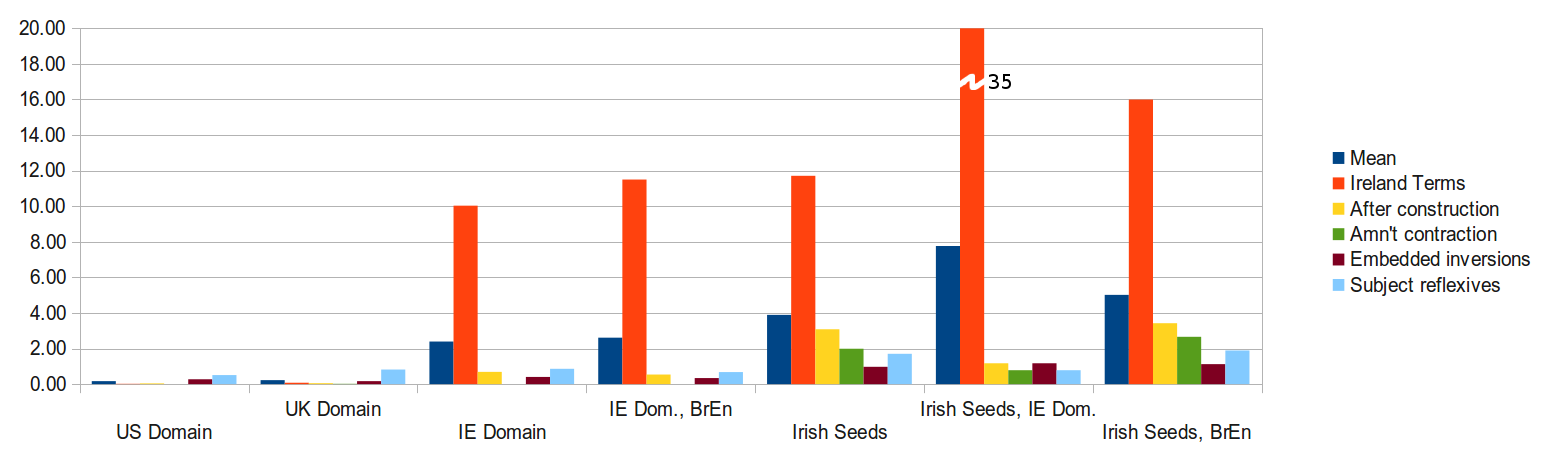
\includegraphics[width=1\textwidth]{characteristicsByCorpus3}
\end{figure*}



\section{Discussion\label{sec:Discussion}}

The results show us that our methods can be effective in extracting
text that is both specific to Irish topics, and includes instances
of constructions that are particular to the variety of English spoken
in Ireland. The incidences relative to corpus size are not as high
as those seen in the manually constructed ICE-Ireland corpus. Currently
we can only speculate on the reasons for this. It may be in part due
to {}``pollution'' of our corpus with non-Irish English, via syndicated
journalism (e.g. some Irish newspapers are repackaging of British
newspapers with added Irish content), or via multinational organisations
with bases in Ireland. In our view the main explanatory factor is
that of modality and register. The ICE-Ireland corpus is predominantly
spoken (\textasciitilde{}60\%), with many texts coming from informal
settings (unscripted speeches, face to face and telephone conversations).
One reading of the figures which is consistent with this viewpoint
is that the IE domain corpora contain proportionally more high register,
edited text (e.g. from governmental and commercial organisations,
for which the use of the IE domain may be an important part of corporate
identity), and that the tailored-seed corpora contain more text contributed
by individuals (forums, blogs, etc), for whom domain endings are of
little consequence.

But despite these lower incidences, in absolute terms our corpora
provide many more examples of Hiberno-English than that were hitherto
available. For example the ICE-Ireland corpus contains a total of
seven examples of the {}``after'' construction, while with our Irish-seeds
derived corpus, and using a fairly restrictive query pattern, we isolated
76 examples of this structure. Further the size of these pilot corpora
were kept intentionally limited, a small fraction of the approximately
150 million IE domain pages indexed by Google. Much larger corpora
could be constructed with relative ease, by using a larger seed set,
or with an interactive seed-discovery method, where the text from
the first round of web-harvesting could be analysed to identify further
terms that are comparatively specific to Hiberno-English (relative
to corpora of other varieties of English).

In terms of wider implications, the fact that seeds tailored to a
particular region and language variant are so effective, relative
to brute filtering by domain, is encouraging for dialects and minority
languages that lack a dedicated internet domain. This suggest that
for less-dominant language variants in web-connected countries (e.g.
Scots, Andalusian, Bavarian), large corpora displaying characteristic
features of that variant can be constructed in a simple automatic
manner with minimal supervision (a small set of seeds provided by
native speakers). For minority languages which are more clearly distinct
from their national dominant language (e.g. Gaelic, Basque, Kurdish),
language identification methods would be an obvious alternative, but
in case such algorithms are not available, these techniques could
be applied. Our methods might also prove useful for dialects in which
a standard variant is dominant in the written language (e.g. Arabic,
Chinese). One might expect that the written Arabic in the .ma (Morocco)
domain would differ little from that in the .qa domain (Qatar) despite
the large differences in vernacular speech. Similarly the grammar
and vocabulary of Chinese written in Mainland Chinese, Taiwanese,
Hong Kong and Singaporese domains (ignoring orthography) might be
less representative of the variation in everyday language. The use
of regional slang and proper names may help one to collect more examples
of this more natural language usage, and less of the dominant standard
variant.

\bibliographystyle{apalike}
\bibliography{egon,brian}

\end{document}
